\section{Introdução}
No anterior artigo desta série vimos como representar uma função periódica como soma de harmónicos, ideia que foi desenvolvida por Fourier quando quis explicar como se propagava o calor. No entanto, essa técnica resultou ser facilmente extrapolável a problemas de outros ramos da física e da engenharia, como a teoria de circuitos elétricos.

Ao longo deste artigo, vamos aplicar a estratégia que desenvolveu Fourier a um clássico problema de eletromagnetismo, o circuito RLC (resistor-indutor-capacitor circuito. De facto, após uma primeira aproximação utilizando senos e cossenos, voltaremos a olhar para o problema sob o prisma da análise complexa, vendo como o problema se simplifica ainda mais.

Se quiserem ampliar, recomendamos que consultem \cite{Sadiku}, uma vez que é o livro que vamos seguir neste artigo.

\section{O circuito RLC}
Vamos começar a colocar detalhadamente o problema que queremos resolver. Temos o circuito mostrado na Figura \ref{fig:RLC}, formado por uma resistência que denotamos por $R$, uma bobina com indução $L$ e um condensador com capacidade $C$, com todos os elementos dispostos em série.
\begin{figure}[h]
\begin{figurebox}
    \vspace{5pt}
    \centering
         \scalebox{1}{%
%
% Com isto ajusto o tamanho dos componentes
\ctikzset{ bipoles/length=1.3cm}
\begin{circuitikz}[scale=1]%\shorthandoff{>}
% Ramo esquerda
    \def\xa{0}
    \def\ya{0}
    \def\xb{1.5}
    \def\yb{3}
    \draw                                     (\xa,\ya)
             to[american voltage source]      (\xa,\yb)
             to[short, -*]                    (\xb,\yb)
             to[open]                         (\xb,\ya)
             to[short, *-]                    (\xa,\ya);
%
%
% Bloco central
    \def\xc{8}
    \def\yc{3.5}
    \def\yd{-0.3}
    \draw [dotted]                            (\xb,\yc)
             to[dotted]                       (\xc,\yc)
             to[dotted]                       (\xc,\yd) 
             to[dotted]                       (\xb,\yd) 
             to[dotted]                       (\xb,\yc);
%
%
% Parte RLC
    \def\xR{4}
    \def\xL{6}
    \def\xC{7}
    \draw                                     (\xb,\yb)
             to[R, l_=$R$]                    (\xR,\yb)
             to[L, l_=$L$]                    (\xL,\yb)
             to                               (\xC,\yb)
             to[C, l_=$C$]                    (\xC,\ya)
             to                               (\xb,\ya);
    \draw                                     (\xC,\yb)
             to                               (\xc,\yb);
    \draw                                     (\xC,\ya)
             to                               (\xc,\ya);
%
%
% Ramo direito
    \def\xd{9}
    \draw                                     (\xc,\yb)
             to[short,*-]                     (\xd,\yb)
             to[open,o-o]                     (\xd,\ya) node[right=8pt, above=78pt]{$+$} node[right=8pt, above=-7pt]{$-$}
             to[short,-*]                     (\xc,\ya);
             
%
%
% Símbolo de potencial
    \draw 
    [decorate,decoration={brace,amplitude=5pt},xshift=0pt,yshift=0pt, thick]
    (\xd+0.5,\yb) -- (\xd+0.5,\ya)
    node [black,midway,xshift=25pt] { $v_C(t)$};
%
    \draw [decorate,decoration={brace,amplitude=5pt},xshift=0pt,yshift=0pt, thick, color=white]
    (\xa-1,\ya) -- (\xa-1,\yb)
    node [black,midway,xshift=-6pt] { $V_S(t)$};
\end{circuitikz}}
    \vspace{-5pt}
    \caption{Circuito RLC}
    \label{fig:RLC}
\end{figurebox}
\end{figure}


O circuito é excitado com um sinal $V_S$ que supomos conhecido, e o objetivo é determinar o potencial entre as placas do condensador, ao qual chamaremos $v_C$.

Em geral, a resolução de um circuito elétrico está associada à resolução de uma equação diferencial que temos que deduzir aplicando alguma lei física. Neste caso utilizamos as \textbf{relações constitutivas} de cada elemento, que são as equações que descrevem como se comportam as resistências, as autoinduções ou os condensadores. Neste caso, se $i(t)$ representa a intensidade de corrente no nosso circuito, deduzirá que:

\begin{itemize}
\item A queda de tensão ao longo da resistência é $v_R(t) = i(t) \cdot R$ pela lei de Ohm.
\item A queda de tensão ao longo da indução é $v_L(t) = L\cdot \frac{\text{d} i}{\text{d}t}(t)$.
\item A queda de tensão ao longo do condensador vem determinada por $i(t) = C\cdot \frac{\text{d}v_C}{\text{d}t}(t)$.
\end{itemize}

Ainda, a lei de Kirchoff diz que a soma de todas essas diferenças de tensão deve ser precisamente igual à excitação, isto é:
\begin{equation}
  \label{eq:RLC1}
  V_{S}(t) = v_{R}(t) + v_{L}(t) + v_{C}(t) = i(t)\cdot R + L\cdot \frac{\text{d}i}{\text{d}t}(t) + v_C(t).
\end{equation}
Para simplificar a equação temos que deixar todas as incógnitas em função de $v_C(t)$, para isso, notemos que:
\begin{equation}
  \label{eq:IntensidadCarga}
  \frac{\text{d}i(t)}{\text{d}t} = C\cdot \frac{\text{d}^2v_C}{\text{d}t^2}(t),
\end{equation}
de modo que podemos substituir \eqref{eq:IntensidadCarga} em \eqref{eq:RLC1} para encontrar
\begin{mybox}\vspace{-5mm}
  \begin{equation}
    \label{eq:RLC}
    L\cdot C\cdot v_C''(t) + R\cdot C\cdot v_C'(t) + v_C(t) = V_S(t)
  \end{equation}
\end{mybox}
que e a equação que vamos tentar resolver. Notemos que já aparecem os produtos $L\cdot C$ e $R\cdot C$, extremamente comuns neste tipo de problemas, razão pela qual é útil habitualmente vê-los como coeficientes que caracterizam o circuito.


\section{Resolução do problema}
Tal e como lhe aconteceu a Fourier quando enfrentou o problema da propagação do calor, nós apenas sabemos resolver a equação \eqref{eq:RLC} quando a excitação $V_S$ é uma função simples, como um harmónico. Nesse caso particular, podemos encontrar uma solução que chamaremos função própria ou \textbf{modo normal}. Portanto, quando tivermos uma superposição de harmónicos, a solução será uma superposição de modos normais.

Na altura de aplicar o processo anterior, podemos estar bastante tiempo com contas e perder a perspetiva do que estamos a fazer, de modo que é conveniente dividir a resolução em três passos, que essencialmente são:
\begin{mybox}
  \begin{enumerate}[{\bfseries [R1]}]
  \item Dividir o problema complicado por vários problemas simples.
  \item Resolver por separado cada um dos problemas simples.
  \item Juntar as soluções para obter a solução do problema complicado.
\end{enumerate}
\end{mybox}

Ora bem, antes de começar a utilizar séries de Fourier, notemos que \eqref{eq:RLC} é uma equação diferencial linear de segunda ordem. Como não é homogénea, sabemos que a solução geral é da forma:
\[
v_C(t) = y_h(t) + y_p(t),
\]
em que $y_h$ é a solução geral da correspondente equação homogénea:
\begin{equation}
  \label{eq:HomogeneaRLC}
  L\cdot C \cdot v_C '' (t) + R\cdot C\cdot v_C'(t) + v_C(t) = 0,
\end{equation}
 entretanto $y_p$ é uma solução particular da não homogénea \eqref{eq:RLC}.

\subsection{Solução de la homogénea} \label{solucionHomogenea}
Como a equação \eqref{eq:HomogeneaRLC} é de coeficientes constantes, as soluções são combinações lineares de funções da forma:
\[
y_h(t) = e^{r\cdot t},
\]
em que $r$ é uma constante que pode ser complexa\footnote{Para uma análise detalhada das equações diferenciais de coeficientes constantes, consultar \cite[p.~226]{DiPrima}}. Ao substituir $y_h$ em \eqref{eq:HomogeneaRLC} deduzimos que $r$ deve ser solução da equação característica
\begin{equation}
  \label{eq:Característica}
  L\cdot C\cdot r^2 + R\cdot C\cdot r + 1 = 0
\end{equation}
de modo que o problema passa por analisar esta equação de segundo grau. Despejando $r$ de \eqref{eq:Caracteristica} obtemos:
\[
r_\pm = -\frac{R}{2\cdot L} \pm \sqrt{\left( \frac{R}{2\cdot L} \right)^2 - \frac{1}{L\cdot C}} \equiv \alpha \pm \sqrt{\Delta},
\]
a depender do signo de
\[
\Delta = \left( \frac{R}{2\cdot L} \right)^2 - \frac{1}{L\cdot C},
\]
podemos obter valores de $r$ reais ou complexos, e em cada caso vamos obter uma solução ligeiramente diferente.
\begin{itemize}
  \item Se $\Delta > 0$, então temos dois valores reais $r_{\pm}=\alpha \pm \beta $, de modo que podemos pôr:
\[
y_h(t) = C_{\!_+} e^{r_{\!_+} t} + C_{\!_-} e^{r_{\!_-}t} = e^{\alpha t}\left(C_1\sinh(\beta\, t) + C_2 \cosh(\beta\, t)\right).
\]
Dizemos que neste caso temos \textbf{amortecimento supercrítico}, uma vez que a solução tende para zero sem oscilar conforme o tempo aumenta.
  \item Se $\Delta = 0$, então temos uma solução real dupla $r$, portanto:
\[
y_h(t) = (C_1t+C_2)\cdot e^{rt}.
\]
Neste caso temos \textbf{amortecimento crítico}, situação em que a solução converge a zero mais rapidamente.
  \item Se $\Delta < 0$, então temos dois valores complexos conjugados $r_{\pm}=\alpha \pm i\beta$, e podemos escrever:
\[
y_h(t) = C_{\!_+} \cdot e^{r_{\!_+}  t} + C_{\!_-}\cdot  e^{r_{\!_-} t} = e^{\alpha t}\cdot \left(C_1\cdot \sin(\beta\, t) + C_2 \cdot \cos(\beta\, t)\right).
\]
Este caso é conhecido como \textbf{amortecimento subcrítico}, uma vez que el amortecimento não é suficiente para evitar que a solução fique oscilando.
\end{itemize}

\begin{figure}
\begin{figurebox}
    \vspace{10pt}
    \centering
      \begin{subfigure}{.3\textwidth}
          \centering
          \scalebox{0.25}{ \input{CodigosDibujos/OverDamped.tex}}
          \caption{$\Delta>0$}
          \label{fig:0a} 
      \end{subfigure} %
      \begin{subfigure}{.3\textwidth}
          \centering
          \scalebox{0.25}{% Title: glps_renderer figure
% Creator: GL2PS 1.3.8, (C) 1999-2012 C. Geuzaine
% For: Octave
% CreationDate: Wed Jul  2 10:01:39 2014
\setlength{\unitlength}{1pt}
\begin{picture}(0,0)
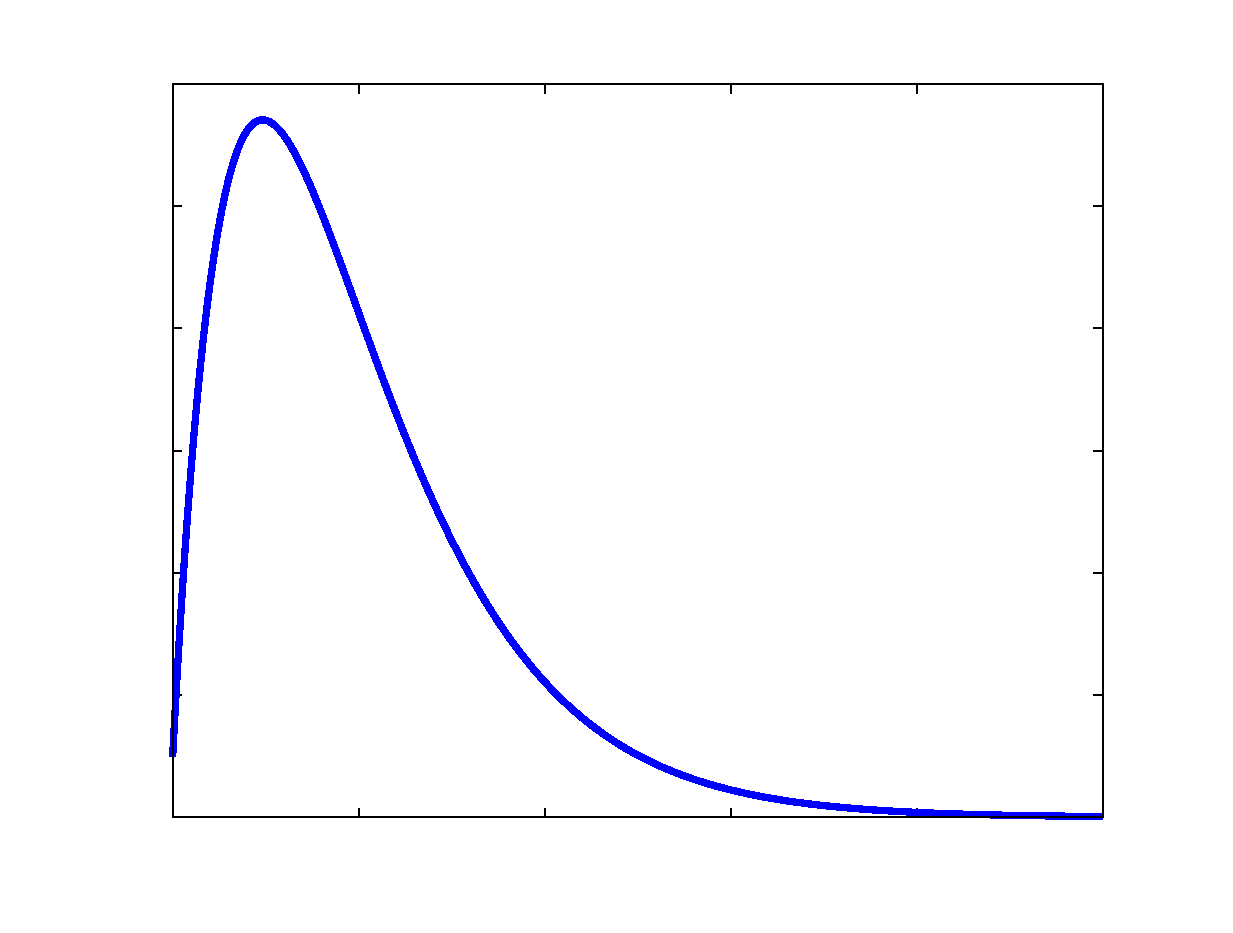
\includegraphics{CriticallyDamped-inc}
\end{picture}%
\begin{picture}(576,432)(0,0)
\fontsize{10}{0}
\selectfont\put(74.8799,42.519){\makebox(0,0)[t]{\textcolor[rgb]{0,0,0}{{0}}}}
\fontsize{10}{0}
\selectfont\put(164.16,42.519){\makebox(0,0)[t]{\textcolor[rgb]{0,0,0}{{20}}}}
\fontsize{10}{0}
\selectfont\put(253.44,42.519){\makebox(0,0)[t]{\textcolor[rgb]{0,0,0}{{40}}}}
\fontsize{10}{0}
\selectfont\put(342.72,42.519){\makebox(0,0)[t]{\textcolor[rgb]{0,0,0}{{60}}}}
\fontsize{10}{0}
\selectfont\put(432,42.519){\makebox(0,0)[t]{\textcolor[rgb]{0,0,0}{{80}}}}
\fontsize{10}{0}
\selectfont\put(521.28,42.519){\makebox(0,0)[t]{\textcolor[rgb]{0,0,0}{{100}}}}
\fontsize{10}{0}
\selectfont\put(69.8755,47.52){\makebox(0,0)[r]{\textcolor[rgb]{0,0,0}{{0}}}}
\fontsize{10}{0}
\selectfont\put(69.8755,106.2){\makebox(0,0)[r]{\textcolor[rgb]{0,0,0}{{2}}}}
\fontsize{10}{0}
\selectfont\put(69.8755,164.88){\makebox(0,0)[r]{\textcolor[rgb]{0,0,0}{{4}}}}
\fontsize{10}{0}
\selectfont\put(69.8755,223.56){\makebox(0,0)[r]{\textcolor[rgb]{0,0,0}{{6}}}}
\fontsize{10}{0}
\selectfont\put(69.8755,282.24){\makebox(0,0)[r]{\textcolor[rgb]{0,0,0}{{8}}}}
\fontsize{10}{0}
\selectfont\put(69.8755,340.92){\makebox(0,0)[r]{\textcolor[rgb]{0,0,0}{{10}}}}
\fontsize{10}{0}
\selectfont\put(69.8755,399.6){\makebox(0,0)[r]{\textcolor[rgb]{0,0,0}{{12}}}}
\end{picture}
}
          \caption{$\Delta=0$}
          \label{fig:0b}
      \end{subfigure} %
      \begin{subfigure}{.3\textwidth}
          \centering
          \scalebox{0.25}{\input{CodigosDibujos/UnderDamped.tex}}
          \caption{$\Delta<0$}
          \label{fig:0c}
      \end{subfigure}
      % 
      \caption{Tipo de soluções da equação homogénea ($y_h$) a depender do signo de $\Delta$.}
      \label{fig:SolucionesHomogenea}
    
\end{figurebox}
\end{figure}

Para terminar de concretizar a solução, apenas é necessário dar determinados valores às constantes. Estes valores devem ser escolhidos de forma a se cumprirem as condições iniciais que impõe o circuito. Para isso, devem ter-se em conta as exigências físicas dos elementos que temos, como a indução e o condensador. Em qualquer caso, não nos interessa fazer essa análise agora.


\subsection{Solução da não homogénea} 
É o momento de resolver a equação \eqref{eq:RLC}, de modo que procuramos uma função_p$ que satisfaça a equação \eqref{eq:RLC}, portanto tem que ser:
\[
L\cdot C \cdot y_p '' (t) + R\cdot C\cdot y_p'(t) + y_p(t) = V_S(t).
\]
Como antecipávamos, não podemos tentar resolver a equação se não nos dizerem mais nada sobre $V_S$, portanto vamos ter que recorrer às séries de Fourier, seguindo os três passos que estabelecemos anteriormente.

\begin{enumerate}[{\bfseries [1]}]
  \item\textit{\color{blue} Dividir o problema complicado por vários problemas simples.}

    Em primeiro lugar, o sinal de excitação \textbf{real} vai ser sempre finita, de modo que apenas me interessa $V_S(t)$ num determinado intervalo de tempo. Ora bem, a função matemática que utilizamos para representar o sinal pode-se \textit{estender} a uma função periódica (a ideia para o conseguir é ir repetindo a gráfica para os lados).

Com este esclarecimento estamos em condições de aplicar o teorema de Fourier. Se $V_S$ tem período $2p$ podemos escrevê-lo como soma de harmónicos:
\[
V_S(t) = a_0 + \sum_{k=0}^{\infty} [a_k \cdot \cos(\omega_kt) + b_k \cdot \sin(\omega_kt)]\qquad \text{donde}\quad \omega_k=\frac{k\cdot \pi}{p}.
\]
  \item \textit{\color{blue}Resolver por separado cada um dos problemas simples.}

Colocamos por separado o caso em que $V_S$ é uma constante, ou uma soma de cossenos e senos.

 $\clubsuit$ Vamos encontrar $y_0$, solução de:
\[
L\cdot C \,y_0 '' (t) + R\cdot C\, y_0'(t) + y_0(t) = a_0.
\]
Neste caso, é fácil ver que
\[\boxed{
y_0(t) = a_0
}\]
cumpre os requisitos.

 $\clubsuit$ Agora vamos encontrar $y_{k}$, solução de:
\[
L\cdot C \,y_k '' (t) + R\cdot C\, y_k'(t) + y_k(t) = a_k\cdot \cos(\omega_kt) +  b_k\cdot \sin(\omega_kt) .
\]
Nestes casos, a literatura sugere experimentar uma solução da forma:
\[
y_{k}(t) = \alpha_k\cdot \cos(\omega_kt) + \beta_k\cdot \sin(\omega_kt),
\]
em que $\alpha_k$ y $\beta_k$ são coeficientes por determinar. Definimos agora:
\[
A_k = 1- L\cdot C\omega_k^2,\qquad\text{y}\qquad B_k = R\cdot C\omega_k.
\]
Estes coeficientes são úteis porque se derivamos $y_{k}$ e substituímos na equação diferencial, obtemos:
\[
 \left[A_k \cdot \alpha_k + B_k\cdot \beta_k\right] \cos(\omega_k t) + \left[-B_k \cdot \alpha_k + A_k\cdot \beta_k\right] \sin(\omega_k t) = a_k\cdot \cos(\omega_kt) +  b_k\cdot \sin(\omega_kt) ,
\]
de modo que a função proposta será solução precisamente quando os coeficientes cumprirem o seguinte sistema de equações que podemos escrever e resolver matricialmente
\[
\left(\begin{array}{cc}
A_k  & B_k\\
-B_k & A_k
\end{array}\right)
\left(\begin{array}{c}
 \alpha_k  \\
 \beta_k
\end{array}\right)
=
\left(\begin{array}{c}
 a_k  \\
 b_k
\end{array}\right)
%
\quad \Longrightarrow \quad
%
\left(\begin{array}{c}
 \alpha_k  \\
 \beta_k
\end{array}\right)
=
\frac{1}{A_k^2+B_k^2}
\left(\begin{array}{c}
 a_k\cdot A_k-b_k\cdot B_k \\
 a_k\cdot B_k + b_k\cdot A_k
\end{array}\right).
\] 
Portanto, a solução fica:
\begin{equation}
  \label{eq:ModoNormal}
  \boxed{
    y_k(t) = \frac{a_k\cdot A_k-b_k\cdot B_k}{A_k^2+B_k^2}\cos(\omega_kt) + \frac{a_k\cdot B_k + b_k\cdot A_k}{A_k^2+B_k^2}\sin(\omega_kt).
  }
\end{equation}

Cada uma destas soluções recebe o nome de \textbf{modo normal de ordem $\mathbf{k}$}.
 
  \item \textit{\color{blue}Juntar as soluções para obter a solução do problema complicado.}

Basta considerar
\[\boxed{
y_p (t)= \sum _{k=0}^{\infty} y_k (t),
}\]
que por construção, é a solução particular que procurávamos.
\end{enumerate}

\subsection{Interpretação  das soluções}
Como já foi mencionado antes, a solução de \eqref{eq:RLC} é soma de duas contribuições:
\[
v_C(t) = y_h(t) + y_p(t),
\]
que podemos analisar por separado:
\begin{itemize}
  \item $y_h(t)$ conhece-se como \textbf{resposta natural ou transitória} (agora veremos porquê). É a contribuição inerente ao próprio circuito e aos elementos que o compõem, uma vez que não depende em absoluto de $V_S$.
  \item $y_p(t)$ conhece-se como \textbf{resposta forçada}. É a resposta que provocamos no circuito por causa da excitação introduzida.
\end{itemize}
De um ponto de vista prático, podemos pensar que temos um \textit{input} $V_S$ ao qual queremos aplicar uma transformação para obter $y_p$. No entanto, o simples facto de utilizar o circuito faz com que o \textit{output} $v_C$ tenha uma contribuição extra $y_h$. Ora bem, resulta que $y_h$ se torna desprezível à medida que passa o tempo, mais explicitamente:
\[
\lim _{t\rightarrow \infty} y_h (t) = 0,
\]
como se pode comprovar fazendo os correspondentes limites ou vendo os exemplos da Figura \ref{fig:SolucionesHomogenea}. Em consequência
\begin{equation}
  \label{eq:aproximacionSolucionRLC}
  v_C(t) \approx y_p(t)\qquad \text{si }t \text{ é suficientemente grande}.
\end{equation}

Como temos que esperar até alcançar uma solução que se estabilize no tempo, dizemos que estamos perante um  \textbf{fenómeno transitório}. A Figura \ref{fig:Transitorio} ilustra esta situação, em que o sinal triangular à saída vê-se alterado nos primeiros instantes.

\begin{figure}
\begin{figurebox}
    \vspace{0pt}
    \centering
    \scalebox{0.4}{ % Title: glps_renderer figure
% Creator: GL2PS 1.3.8, (C) 1999-2012 C. Geuzaine
% For: Octave
% CreationDate: Mon Jul  7 19:08:28 2014
\setlength{\unitlength}{1pt}
\begin{picture}(0,0)
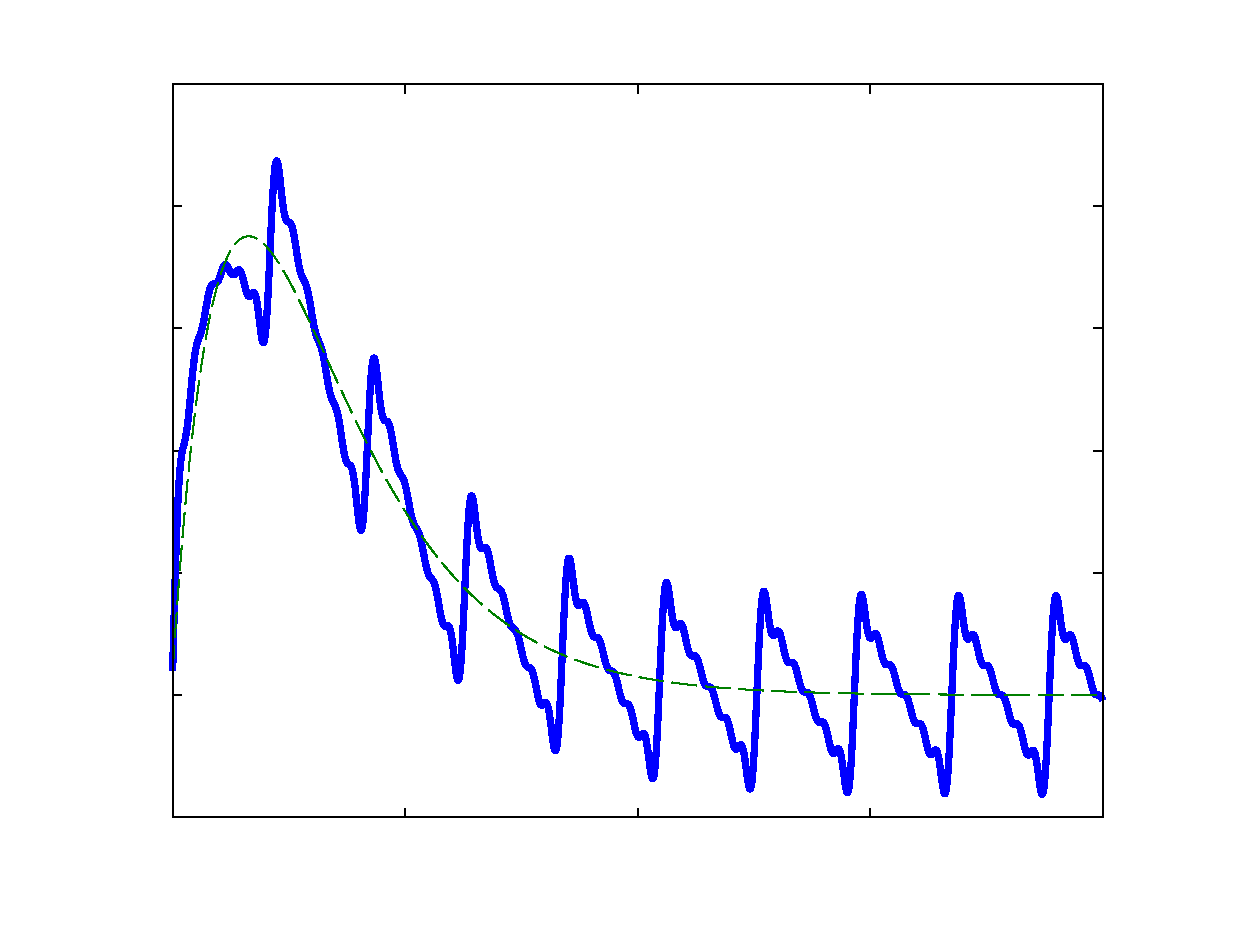
\includegraphics{SumaSoluciones-inc}
\end{picture}%
\begin{picture}(576,432)(0,0)
\fontsize{10}{0}
\selectfont\put(74.8799,42.519){\makebox(0,0)[t]{\textcolor[rgb]{0,0,0}{{0}}}}
\fontsize{10}{0}
\selectfont\put(186.48,42.519){\makebox(0,0)[t]{\textcolor[rgb]{0,0,0}{{50}}}}
\fontsize{10}{0}
\selectfont\put(298.08,42.519){\makebox(0,0)[t]{\textcolor[rgb]{0,0,0}{{100}}}}
\fontsize{10}{0}
\selectfont\put(409.68,42.519){\makebox(0,0)[t]{\textcolor[rgb]{0,0,0}{{150}}}}
\fontsize{10}{0}
\selectfont\put(521.28,42.519){\makebox(0,0)[t]{\textcolor[rgb]{0,0,0}{{200}}}}
\fontsize{10}{0}
\selectfont\put(69.8755,47.52){\makebox(0,0)[r]{\textcolor[rgb]{0,0,0}{{-2}}}}
\fontsize{10}{0}
\selectfont\put(69.8755,106.2){\makebox(0,0)[r]{\textcolor[rgb]{0,0,0}{{0}}}}
\fontsize{10}{0}
\selectfont\put(69.8755,164.88){\makebox(0,0)[r]{\textcolor[rgb]{0,0,0}{{2}}}}
\fontsize{10}{0}
\selectfont\put(69.8755,223.56){\makebox(0,0)[r]{\textcolor[rgb]{0,0,0}{{4}}}}
\fontsize{10}{0}
\selectfont\put(69.8755,282.24){\makebox(0,0)[r]{\textcolor[rgb]{0,0,0}{{6}}}}
\fontsize{10}{0}
\selectfont\put(69.8755,340.92){\makebox(0,0)[r]{\textcolor[rgb]{0,0,0}{{8}}}}
\fontsize{10}{0}
\selectfont\put(69.8755,399.6){\makebox(0,0)[r]{\textcolor[rgb]{0,0,0}{{10}}}}
\end{picture}
}
    \vspace{-10pt}
    \caption{Fenómeno transitório}
    \label{fig:Transitorio}
\end{figurebox}
\end{figure}





\subsection{Solução final}
Depois de todo o trabalho, já podemos dar uma fórmula fechada para a solução de \eqref{eq:RLC}.
\begin{mybox} \vspace{-4mm}
  \begin{equation}
    \label{eq:SolucionRLC}
    v_C(t) = y_h(t) + \sum _{k=0}^{\infty} y_k (t) = y_h(t) +  \sum _{k=0}^{\infty}  \frac{a_k\cdot A_k-b_k\cdot B_k}{A_k^2+B_k^2}\cos(\omega_kt) + \frac{a_k\cdot B_k + b_k\cdot A_k}{A_k^2+B_k^2}\sin(\omega_kt),
  \end{equation}
  em que $y_h(t)$ é uma das três opções descritas na secção \ref{solucionHomogenea}.
\end{mybox}

Notemos que pusemos a mesma fórmula para o caso $k=0$, dado que nesse caso a excitação é constante, isso equivale a tomar certo $\omega_0=0$ e recupera-se precisamente $y_0=a_0$.

Já precisámos que $y_h(t)$ se torna desprezível à medida que passa o tempo, portanto também vamos deixar escrita a solução \textit{estável no tempo}.

\begin{mybox} \vspace{-4mm}
  \begin{equation}
    \label{eq:SolucionRLC2}
    v_C(t) \approx \sum _{k=0}^{\infty}  \frac{a_k\cdot A_k-b_k\cdot B_k}{A_k^2+B_k^2}\cos(\omega_kt) + \frac{a_k\cdot B_k + b_k\cdot A_k}{A_k^2+B_k^2}\sin(\omega_kt).
  \end{equation}
\end{mybox}


\section{Enfoque complexo}

No anterior artigo descobrimos a relação entre exponenciais complexas e harmónicos. Agora vamos explorar como levar a cabo a resolução do circuito tirando proveito desta ideia, chegando ao extremo de não ter que resolver nenhuma equação diferencial. Ora bem, este método apenas nos permite obter uma solução particular e não tem em consideração as condições iniciais.

Antes de começar, é necessário fazer uma precisão. Quando se trabalha com circuitos elétricos, é comum representar a unidade imaginária com a letra $j$ para evitar uma possível confusão com a intensidade $i(t)$. Desta forma, escreveremos um número complexo arbitrário como $a+jb\in\mathbb{C}$.

O que é que acontece se, por um momento, imaginamos que temos um sinal complexo da forma $e^{i\omega t}$? Evidentemente, este não será nunca o caso dado que os sinais são reais, mas já sabemos que um sinal real se pode pôr como soma de exponenciais complexas, portanto a nossa pergunta faz sentido. Sob esta premissa, nasce a ideia de fasor, que analisamos a seguir.

\subsection{Fasores}
Como já vimos, é muito comum trabalhar com harmónicos na altura de analisar circuitos elétricos. Ora bem, uma tensão da forma $v(t) = V \cos(\omega t + \phi)$ pode relacionar-se com exponenciais complexas através de
\[
v(t) = \frac{V\cdot e^{j(\omega t + \phi)} + V\cdot e^{-j(\omega t + \phi)}}{2}.
\]
Mas por enquanto vamos utilizar uma outra relação completamente equivalente que servirá melhor para o nosso propósito:
\[
v(t) = \operatorname{Re} \left[V \cdot e^{j(\omega t + \phi)}\right] = \operatorname{Re} \left [V \cdot e^{j\phi} e^{j\omega t}\right] = \operatorname{Re} \left[\mathbf{V} \cdot  e^{j\omega t}\right],
\]
em que $\mathbf{V} = V \cdot e^{j\phi}$ recebe o nome de \textbf{fasor}, e é uma quantidade complexa que representa o sinal. Como vemos, o fasor apenas nos diz a amplitude e a fase de um harmónico. A dependência temporária mantém-se separada mediante o termo $e^{j\omega t}$.

Para a intensidade que circula pelo circuito podemos utilizar o mesmo critério\footnote{Se a tensão é um harmónico, também o é a intensidade, consequência das relações constitutivas de cada elemento (ver \cite{FasorIntensidad}).} e representá-la por meio do fasor $\mathbf{I}$, sabendo que podemos recuperar o valor real como $i(t)=\operatorname{Re}\left[\mathbf{I}\cdot e^{j\omega t}\right]$.

Que vantagens apresenta isto? Vamos ver como expressar as relações constitutivas de cada elemento neste contexto.

\begin{itemize}
  \item Quando há uma resistência, tem-se uma queda de tensão $v_R$ dada por:
    \[
    v_R(t) = i(t)\cdot  R = \operatorname{Re}\left[\mathbf{I}\cdot e^{j\omega t}\right]\cdot R = \operatorname{Re}\left[R\cdot \mathbf{I}\cdot e^{j\omega t}\right],
    \]
    de modo que à tensão $v_R$ lhe podemos associar um fasor relacionado com o da intensidade por meio de
    \begin{equation}
      \label{eq:FasorVR}
      \mathbf{V}_R = R\cdot \mathbf{I}.
    \end{equation}

  \item Quando há uma indução no circuito, a queda de tensão que apresenta $v_L$ vem dada por:
    \[
    v_L(t) = L \cdot \frac{\text{d}i}{\text{d}t}(t) = L \cdot \operatorname{Re} \left[\frac{\text{d} (\mathbf{I}\cdot e^{j\omega t})}{\text{d}t}\right] = L \cdot  \operatorname{Re} \left[j\cdot \omega\cdot \mathbf{I}\cdot e^{j\omega t}\right] =   \operatorname{Re} \left[j\cdot \omega L\cdot \mathbf{I} \cdot e^{j\omega t}\right],
    \]
    de modo que à tensão $v_L$ lhe podemos associar um fasor relacionado com o da intensidade por meio de
    \begin{equation}
      \label{eq:FasorVL}
      \mathbf{V}_L = j \cdot \omega \cdot L\cdot\mathbf{I}.
    \end{equation}

  \item Quando há um condensador no circuito, a queda de tensão que apresenta $v_C$ vem dada por:
    \[
    v_C(t) = \frac{q(t)}{C} \quad \Longrightarrow \quad  \frac{\text{d}v}{\text{d}t}(t) = \frac{i(t)}{C}  \quad \Longrightarrow \quad \operatorname{Re}\left[j\cdot \omega\cdot \mathbf{V}_C\cdot e^{j\omega t}\right] = \operatorname{Re} \left[\frac{\mathbf{I}\cdot e^{j\omega t}}{C}\right],
    \]
    de forma que à tensão $v_C$ lhe podemos associar um fasor relacionado com o da intensidade por meio de
    \begin{equation}
      \label{eq:FasorVC}
      \mathbf{V}_C = \frac{1}{j\cdot  \omega \cdot C}\,\mathbf{I}.
    \end{equation}
\end{itemize}

\subsection{Impedância}
Agora que temos os fasores como nova ferramenta, podemos utilizá-la para expressar de novo a lei de Kirchoff:
\begin{equation}
  \label{eq:KirchoffFasores}
  \mathbf{V}_R + \mathbf{V}_L + \mathbf{V}_C = \mathbf{V}_S,
\end{equation}
e substituindo as relações \labelcref{eq:FasorVR,eq:FasorVL,eq:FasorVC} em \eqref{eq:KirchoffFasores} encontramos
\[
  \left(R + j\cdot \omega \cdot L + \frac{1}{j\cdot \omega \cdot C}\right) \mathbf{I} = \mathbf{V}_S.
\]
O que nos sugere definir o número complexo
\begin{equation}
  \label{eq:Impedancia}
  \mathbf{Z}=\frac{\mathbf{V}_S}{\mathbf{I}} = R + j\cdot \omega \cdot L + \frac{1}{j\cdot \omega \cdot C},
\end{equation}
conhecido como \textbf{impedência}. Em geral, define-se a impedância $\mathbf{Z}$ de um circuito ou um elemento como o número (geralmente complexo) que satisfaz:
\begin{equation}
  \label{eq:OhmGeneral}
  \mathbf{V} = \mathbf{I}\cdot \mathbf{Z}.
\end{equation}
Desta forma, podemos entender a impedância como uma generalização do conceito de resistência, mas englobando também condensadores e indutores. Portanto, podemos ver também \eqref{eq:OhmGeneral} como uma extensão da lei de Ohm. 

Aqui é onde estão a começar a aparecer as diferenças essenciais. Ao passar-nos para o campo complexo, estamos a enfrentar um problema em que todos os elementos se comportam essencialmente como resistências, o que faz com que a sua resolução seja trivial. Ainda, o potencial deste método radica na sua generalidade, uma vez que podemos repeti-lo \textbf{para qualquer circuito}.


\subsection{Resolução}
 Recordemos que o nosso objetivo era encontrar a tensão entre as placas do condensador, para isso substituímos \eqref{eq:Impedancia} em \eqref{eq:FasorVC}, obtendo:
\begin{equation}
  \label{eq:SolFasor}
  \mathbf{V}_C = \frac{1}{j\cdot \omega \cdot C} \frac{\mathbf{V_S}}{\mathbf{Z}} =\frac{\frac{1}{j\cdot \omega\cdot C}}{R + j\cdot \omega \cdot L + \frac{1}{j\cdot \omega \cdot C}} \mathbf{V}_S = \frac{1}{(1-\omega^2 \cdot L\cdot C) + j(\omega\cdot R\cdot  C)} \mathbf{V}_S.
\end{equation}

Donde deduziríamos $v_C(t) = \operatorname{Re} \left[\mathbf{V}_C \cdot e^{j\omega t}\right]$. Como isto é válido apenas se a tensão de excitação é uma exponencial complexa, em caso real necessitamos aplicar de novo a nossa estratégia.

\begin{enumerate}[{\bfseries [1]}]
  \item\textit{\color{blue} Dividir o problema complicado por vários problemas simples.}

    Para uma excitação genérica, encontramos a sua série de Fourier complexa:
    \[
    V_S(t) = \sum_{k=-\infty}^\infty c_k \cdot e^{j\omega_k t},
    \]
    e já temos a excitação como soma de exponenciais complexas. Cada uma delas pode ser representada mediante o fasor $c_k$.
  \item \textit{\color{blue}Resolver por separado cada um dos problemas simples.}

    Para cada contribuição, tomamos o seu fasor e com \eqref{eq:SolFasor} obtemos o fasor da solução, donde:
    \[\boxed{
      \tilde{y}_k (t)= \operatorname{Re}\left[\frac{1}{(1-\omega_k^2 \cdot  L\cdot C) + j(\omega_k R\cdot C)}\ c_k\cdot  e^{j\omega_k t}\right].
    }\]
  \item \textit{\color{blue}Juntar as soluções para obter a solução do problema complicado.}

    Simplesmente é suficiente fazer
    \[
    v_C(t) =  \sum_{k=-\infty}^\infty \tilde{y}_k(t) = \operatorname{Re}\left[\ \sum_{k=-\infty}^\infty \frac{1}{(1-\omega_k^2 \cdot L\cdot C) + j(\omega_k\cdot R\cdot C)}\cdot  c_k\cdot e^{j\omega_k t}  \right].
    \] 
    Finalmente, os termos com índices $k$ e $-k$ são conjugados\footnote{Com efeito, é suficiente recordar que $c_{-k} = \overline{c_k}$, $\omega_{-k}=-\omega_k$ e que $\overline{e^z}=e^{\overline{z}}$}, portanto a soma é um número real e é suficiente pôr
    \begin{equation} \boxed{
      \label{eq:SolucionFasores}
      v_C(t) = \sum_{k=-\infty}^\infty \frac{1}{(1-\omega_k^2 \cdot L\cdot C) + j(\omega_k\cdot R\cdot C)}\cdot c_k \cdot e^{j\omega_k t}.
    } \end{equation}
\end{enumerate}




\subsection{Solução final}
O que nos permitiu resolver o problema com rapidez foi trabalhar no \textbf{domínio fasorial} ou \textbf{domínio da frequência}. Após ter feito isso, é trivial encontrar \eqref{eq:SolFasor}, e a partir daí construir a solução \eqref{eq:SolucionFasores}, que ganha em simplicidade dado que nos desprendemos de ter que considerar partes reais. Simplesmente é suficiente multiplicar cada exponencial por uma impedância e somá-las.

Como dizíamos, este método apenas nos proporciona uma solução particular, para a qual podemos dar a seguinte fórmula fechada:
\begin{mybox} \vspace{-4mm}
  \begin{equation}
    \label{eq:SolucionRLC3}
    v_C(t) = \sum_{k=-\infty}^\infty \frac{1}{(1-\omega_k^2 \cdot L\cdot C) + j(\omega_k \cdot R\cdot C)}\cdot c_k \cdot e^{j\omega_k t}.
  \end{equation}
\end{mybox}

Este pode ser um bom momento para comprovar que as soluções \eqref{eq:SolucionRLC2} e \eqref{eq:SolucionRLC3}, obtidas com dois métodos diferentes, são iguais. Para isso, vejamos que $ \tilde{y}_k + \tilde{y}_{-k} = y_k$ sendo $y_k$ o que definimos em \eqref{eq:ModoNormal} como modo normal.

\begin{align*}
   \tilde{y}_k(t) + \tilde{y}_{-k}(t) 
   &= 2 \tilde{y}_k(t) = 2\operatorname{Re}\left[ \frac{1}{A_k + jB_k}\cdot  \left(\frac{a_k-jb_k}{2}\right)\cdot e^{j\omega_k t} \right] = \operatorname{Re}\left[ \frac{A_k-jB_k}{A_k^2 + B_k^2}\cdot \left(a_k-jb_k\right)\cdot e^{j\omega_k t} \right] \\
   &=  \frac{1}{A_k^2 + B_k^2} \cdot \operatorname{Re}\left[ ((A_k\cdot a_k - B_k\cdot b_k) - j(A_k\cdot b_k + B_k\cdot a_k)) \cdot e^{j\omega_k t} \right] \\
   &= \frac{1}{A_k^2 + B_k^2}\cdot \left[ (A_k\cdot a_k - B_k\cdot b_k)\cos(\omega_k t) + (A_k\cdot b_k + B_k\cdot a_k)\sin(\omega_k t) \right]\\
   &= y_k(t),
\end{align*}
donde se deduz imediatamente que
\[
\sum_{k=-\infty}^\infty \tilde{y}_k(t) = \sum_{k=0}^\infty y_k (t),
\]
e que, portanto, as soluções coincidem.















\section{Ressonância}
Para analisar o circuito RLC tivemos que recorrer, por dois caminhos diferentes, às séries de Fourier. Em ambos os casos, a consequência é que a solução se expressa como uma soma infinita de pequenas contribuições, cada uma associada a uma frequência $\omega_k$ diferente.

Existe alguma frequência que contribua mais do que as outras? Para responder a esta pergunta temos que analisar a \textbf{resposta frequencial}. Da equação \eqref{eq:SolFasor} deduz-se que cada frequência vê multiplicada a sua amplitude pelo termo
\begin{equation}
  \label{eq:FuncionTransferencia}
  H(\omega) = \frac{1}{(1-\omega^2 \cdot L\cdot C) + j(\omega \cdot R\cdot C)}.
\end{equation}
A função $H(\omega)$ recebe o nome de \textbf{função de transferência} e indica quanto aumenta cada exponencial após passar pelo circuito. De facto, como $H(\omega)$ é um número complexo, a informação relativa ao tamanho está contida no módulo:
\begin{equation}
  \label{eq:ModuloFuncionTransferencia}
  \left|H(\omega)\right| = \frac{1}{\sqrt{(1-\omega^2\cdot L\cdot C)^2 + (\omega \cdot R\cdot C)^2}}.
\end{equation}

\begin{figure}
\begin{figurebox}
    \vspace{5pt}
    \centering
    \scalebox{0.4}{ % Title: glps_renderer figure
% Creator: GL2PS 1.3.8, (C) 1999-2012 C. Geuzaine
% For: Octave
% CreationDate: Mon Aug 18 14:41:30 2014
\setlength{\unitlength}{1pt}
\begin{picture}(0,0)
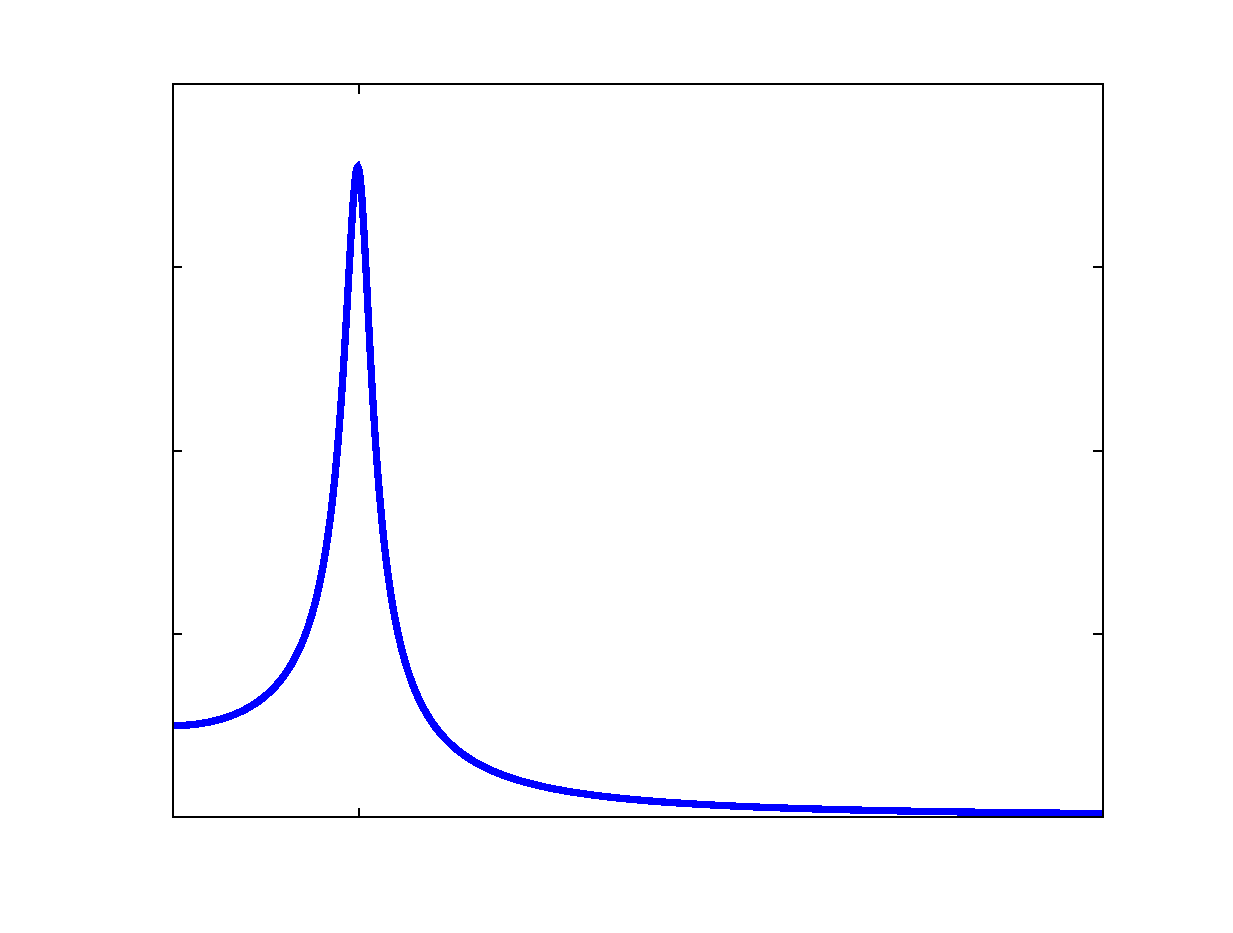
\includegraphics{Resonancia-inc}
\end{picture}%
\begin{picture}(576,432)(0,0)
\fontsize{30}{0}
\selectfont\put(164.16,42.519){\makebox(0,0)[t]{\textcolor[rgb]{0,0,0}{{$\omega_r$}}}}
\fontsize{30}{0}
\selectfont\put(69.8755,47.52){\makebox(0,0)[r]{\textcolor[rgb]{0,0,0}{{0}}}}
\fontsize{30}{0}
\selectfont\put(69.8755,135.54){\makebox(0,0)[r]{\textcolor[rgb]{0,0,0}{{2}}}}
\fontsize{30}{0}
\selectfont\put(69.8755,223.56){\makebox(0,0)[r]{\textcolor[rgb]{0,0,0}{{4}}}}
\fontsize{30}{0}
\selectfont\put(69.8755,311.58){\makebox(0,0)[r]{\textcolor[rgb]{0,0,0}{{6}}}}
\fontsize{30}{0}
\selectfont\put(69.8755,399.6){\makebox(0,0)[r]{\textcolor[rgb]{0,0,0}{{8}}}}
\end{picture}
}
    \vspace{-10pt}
    \caption{Fenómeno de ressonância.}
    \label{fig:Resonancia}
\end{figurebox}
\end{figure}


Na Figura \ref{fig:Resonancia} podemos observar a representação gráfica de \eqref{eq:ModuloFuncionTransferencia}. Como vemos, há uma banda de frequências para as quais $H(\omega)$ é especialmente grande, o que produz o fenómeno conhecido como \textbf{ressonância}. Para caracterizar este fenómeno, define-se a \textbf{frequência de ressonância} como
\begin{equation}
  \label{eq:FrecuenciaNatural}
  \omega_r = \frac{1}{\sqrt{L\cdot C}}.
\end{equation}
Resulta que quando $\omega=\omega_r$ a impedância é um número real e o seu módulo alcança o seu valor mínimo (como se pode comprovar em \eqref{eq:Impedância}), de modo que a intensidade que circula pelo circuito é máxima (consequência imediata de \eqref{eq:OhmGeneral}). Ainda, na prática o coeficiente $R\cdot C$ é muito pequeno, de modo que \eqref{eq:ModuloFuncionTransferencia} alcança o seu valor máximo para uma frequência muito próxima a $\omega_r$.

Por esta e outras razões, a frequência de ressonância é um parâmetro essencial na altura de caracterizar um circuito. A seguir vamos ver uma da suas aplicações mais imediatas.


\subsection{Filtros passabanda}
Quando se trabalha em telecomunicações, é comum encontrar-nos com sinais que apresentam um nível de \textbf{ruído} que nos impede receber o sinal com clareza. Perante esta situação, seria ideal ter alguma forma de eliminar o ruído, fazendo passar o sinal por um \textbf{filtro}.

Para ilustrar esta situação, devemos observar a Figura \ref{fig:EfectoFiltro}, em que representamos o sinal com que começamos e o sinal a que queremos chegar.


\begin{figure}[h]
\begin{figurebox}
    \vspace{10pt}
    \centering
      \begin{subfigure}{.45\textwidth}
          \centering
          \scalebox{0.30}{ \input{CodigosDibujos/SignalRuido.tex}}
          \caption{Sinal sem filtrar}
          \label{fig:0a} 
      \end{subfigure}%
      \begin{subfigure}{.45\textwidth}
          \centering
          \scalebox{0.30}{% Title: glps_renderer figure
% Creator: GL2PS 1.3.8, (C) 1999-2012 C. Geuzaine
% For: Octave
% CreationDate: Wed Jul  9 15:56:49 2014
\setlength{\unitlength}{1pt}
\begin{picture}(0,0)
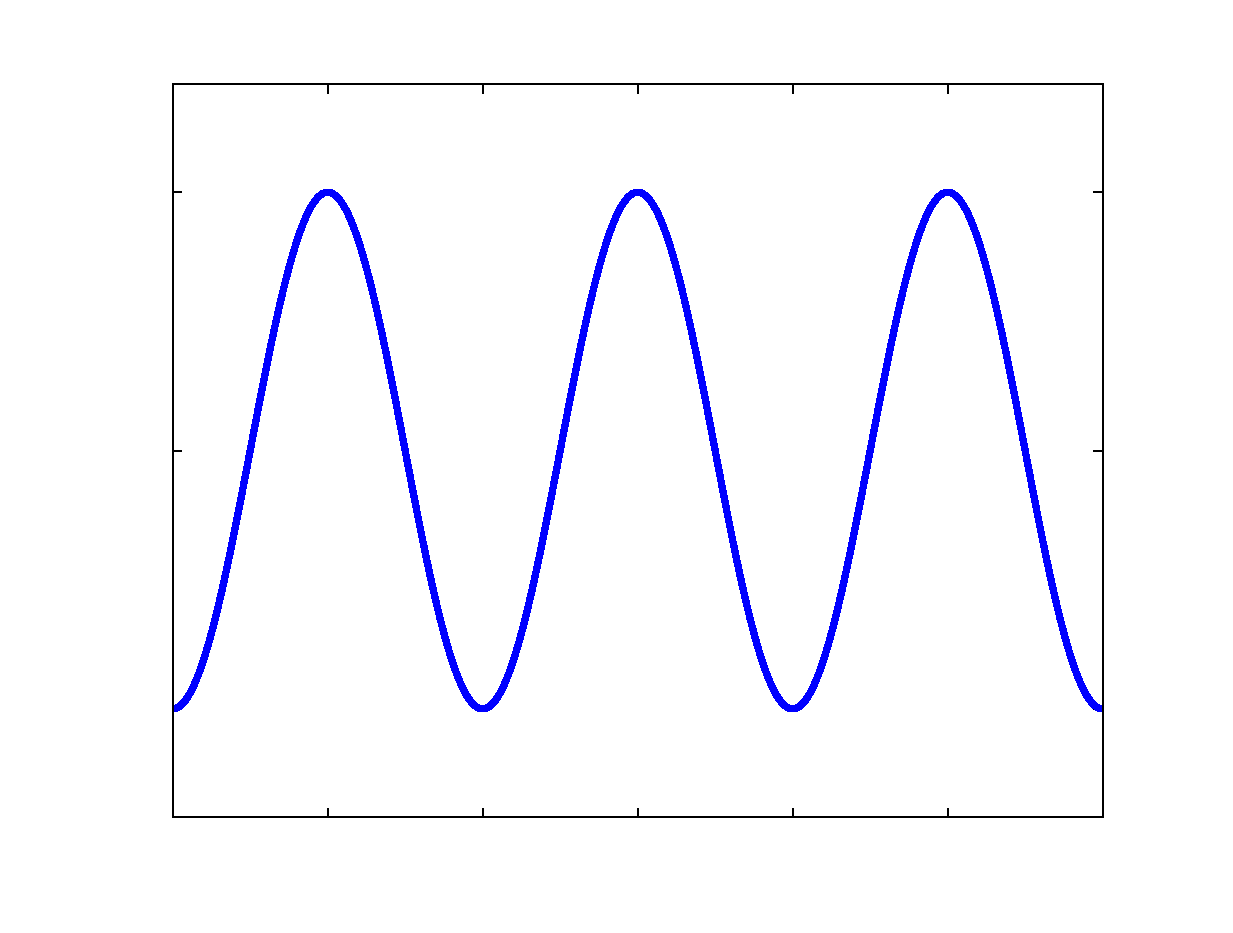
\includegraphics{SignalSinRuido-inc}
\end{picture}%
\begin{picture}(576,432)(0,0)
\fontsize{30}{0}
\selectfont\put(149.28,42.519){\makebox(0,0)[t]{\textcolor[rgb]{0,0,0}{{-2$\pi$}}}}
\fontsize{30}{0}
\selectfont\put(223.68,42.519){\makebox(0,0)[t]{\textcolor[rgb]{0,0,0}{{-$\pi$}}}}
\fontsize{30}{0}
\selectfont\put(298.08,42.519){\makebox(0,0)[t]{\textcolor[rgb]{0,0,0}{{0}}}}
\fontsize{30}{0}
\selectfont\put(372.48,42.519){\makebox(0,0)[t]{\textcolor[rgb]{0,0,0}{{$\pi$}}}}
\fontsize{30}{0}
\selectfont\put(446.88,42.519){\makebox(0,0)[t]{\textcolor[rgb]{0,0,0}{{2$\pi$}}}}
\fontsize{30}{0}
\selectfont\put(69.8755,99.5884){\makebox(0,0)[r]{\textcolor[rgb]{0,0,0}{{-10}}}}
\fontsize{30}{0}
\selectfont\put(69.8755,223.56){\makebox(0,0)[r]{\textcolor[rgb]{0,0,0}{{0}}}}
\fontsize{30}{0}
\selectfont\put(69.8755,347.532){\makebox(0,0)[r]{\textcolor[rgb]{0,0,0}{{10}}}}
\end{picture}
}
          \caption{Sinal filtrado}
          \label{fig:0b}
      \end{subfigure}
      \caption{Efeito do filtro sobre um sinal com ruído}
      \label{fig:EfectoFiltro}
    
\end{figurebox}
\end{figure}

Agora vamos fazer uma suposição essencial: \textit{as frequências que aparecem ao fazer o desenvolvimento de Fourier do ruído não coincidem com as frequências do sinal}. Na prática, nem sempre será legítimo supor isto\footnote{ Em cujo caso, deveria enfrentar-se o problema com uma perspetiva diferente.}, uma vez que depende da natureza do sinal e do tipo de ruído (mais sobre tipos de ruído em \cite{ColorNoise}). Desta maneira, vamos ter uma função à qual podemos fazer o desenvolvimento em série de Fourier, que escrevemos distinguindo explicitamente as frequências que compõem o ruído.
\begin{equation}
  \label{eq:FourierSignalRuido1}
  f(t) = \sum_{\omega_k\text{ de la señal}}\!\!\!\!\!\!\!c_k \cdot e^{j\omega_k t}\ \ +\  \sum_{\omega_k\text{ del ruido}}\!\!\!\!\!c_k \cdot e^{j\omega_k t}.
\end{equation}

Por simplicidade, podemos supor ainda que o primeiro somatório de \eqref{eq:FourierSignalRuido} está composto por um único termo de frequência $\omega_r$, de modo que o desenvolvimento de Fourier fica
\begin{equation}
  \label{eq:FourierSignalRuido}
  f(t) = c_r \cdot e^{j\omega_r t}\ \ +\  \sum_{\omega_k\text{ del ruido}}\!\!\!\!\!c_k \cdot e^{j\omega_k t}.
\end{equation}

Agora é suficiente que façamos passar o sinal por um circuito RLC. Desta forma, o sinal à saída vem dado por \eqref{eq:SolucionRLC3}, e en nesse caso fica:
\begin{equation}
  \label{eq:FourierSignalFiltrada1}
  v_C(t) = H(\omega_r) \cdot c_r \cdot e^{j\omega_r t}\ \ +\  \sum_{\omega_k\text{ del ruido}}\!\!\!\!\! H(\omega_k)\cdot c_k\cdot e^{j\omega_k t}.
\end{equation}
 Ora bem, se escolhemos os valores de $L$ e de $C$ de forma que a frequência $\omega_r$ seja precisamente a frequência de ressonância do circuito (isto é, $\omega_r = \frac{1}{\sqrt{L\cdot C}}$), teremos que:
 \begin{itemize}
 \item $H(\omega_r)$ será relativamente alto (por exemplo, na Figura \ref{fig:Resonancia}, seria $H(\omega_r)\approx 7$).
 \item $H(\omega_k)$ será quase nulo, uma vez que as frequências do ruído estão longe de $\omega_r$. Assim  $H(\omega_k)\approx 0$.
 \end{itemize}
Em consequência temos que o sinal após passar pelo circuito é aproximadamente:
\begin{mybox}\vspace{-15pt}
  \begin{equation}
    \label{eq:FourierSignalFiltrada}
    v_C(t) \approx H(\omega_r) \cdot c_r \cdot e^{j\omega_r t}.
  \end{equation}
\end{mybox}

Por esta razão, dizemos que o circuito funciona como \textbf{filtro}. Em particular, diz-se filtro passabanda porque apenas mantém as frequências que estão numa banda centrada em $\omega_r$ (fora da banda, $H(\omega)\approx 0$). Se o nosso sinal é um pouco mais complicado, seguramente exista um filtro mais complicado que se adapte às nossas necessidades. Alguns exemplos típicos são os filtros passa-baixa, que mantêm todas as frequências abaixo de uma frequência limiar, filtros passa-alta, filtros recusa-banda, bem como combinações dos anteriores.


\bibliographystyle{plain}
\bibliography{fourier1}

\newpage

%%% Local Variables: 
%%% mode: latex
%%% TeX-master: "matematicaseningenieria"
%%% End: 


